
\section{Верификация математической модели}\label{sec:ch2/sec6}
Верификация математической модели  представляет собой неотъемлемый этап разработки, направленный на подтверждение адекватности
и точности полученного математического описания. Процесс верификации включает в себя комплекс методов и подходов,
позволяющих оценить соответствие модели реальному объекту в рамках принятых допущений и ограничений.

Основной целью верификации является подтверждение способности модели корректно отражать физические процессы,
происходящие в электропневматическом приводе, и обеспечивать достоверные результаты при решении задач анализа и синтеза систем управления.
В отсутствие экспериментальных данных, предварительная верификация базируется на теоретическом анализе,
численном моделировании.

Верификация данных происходила на основе следующих параметров модели, которые согласованны
с характерными параметрами экспериментального стенда и представленны в
таблице \ref{tab:ch2/extended_parameters}.

\begin{table}[h]
    \centering
    \caption{Расширенные параметры моделирования электропневматического привода}
    \small
    \begin{tabular}{lccl}
        \textbf{Параметр}                & \textbf{Обозначение}                      & \textbf{Значение}     & \textbf{Размерность} \\
        \midrule
        Масса подвижных частей           & $M$                                       & 6.0                   & кг                   \\
        Ход поршня                       & $L$                                       & 0.3                   & м                    \\
        Диаметр поршня                   & $D_\text{п}$                              & 0.032                 & м                    \\
        Диаметр штока                    & $d_\text{шт}$                             & 0.012                 & м                    \\
        Площадь поршня со стороны штока  & $F_2 = \pi(D_\text{п}^2-d_\text{шт}^2)/4$ & $7.07 \times 10^{-4}$ & м$^2$                \\
        Площадь поршня со стороны крышки & $F_1 = \pi D_\text{п}^2/4$                & $8.04 \times 10^{-4}$ & м$^2$                \\
        Давление питания                 & $p_\text{п}$                              & $6 \times 10^5$       & Па                   \\
        Атмосферное давление             & $p_\text{атм}$                            & $1 \times 10^5$       & Па                   \\
        Газовая постоянная воздуха       & $R$                                       & 287                   & Дж/(кг$\cdot$К)      \\
        Температура воздуха              & $T_\text{атм}$                            & 293                   & К                    \\
        Показатель адиабаты              & $\gamma$                                  & 1.4                   & -                    \\
        Коэффициент расхода              & $C_d$                                     & 0.7                   & -                    \\
        Эффективная площадь клапана      & $A_v$                                     & $1.2 \times 10^{-6}$  & м$^2$                \\
        \midrule
        \multicolumn{4}{l}{\textbf{Параметры силы трения:}}                                                                         \\
        \midrule
        Сила сухого трения               & $F_c$                                     & 50                    & Н                    \\
        Сила трения покоя                & $F_s$                                     & 60                    & Н                    \\
        Коэффициент вязкого трения       & $\sigma_2$                                & 100                   & Н$\cdot$с/м          \\
        Скорость Штрибека                & $v_s$                                     & 0.01                  & м/с                  \\
        Показатель степени Штрибека      & $\delta$                                  & 2                     & -                    \\
        \midrule
        \multicolumn{4}{l}{\textbf{Параметры реакции опор:}}                                                                        \\
        \midrule
        Коэффициент жесткости опоры      & $k_\text{оп}$                             & $1 \times 10^6$       & Н/м                  \\
        Коэффициент демпфирования опоры  & $b_\text{оп}$                             & 1000                  & Н$\cdot$с/м          \\
        Координата нижнего упора         & $x_\text{мин}$                            & 0                     & м                    \\
        Координата верхнего упора        & $x_\text{макс}$                           & 0.3                   & м                    \\
        \midrule
    \end{tabular}
    \label{tab:ch2/extended_parameters}
\end{table}

\subsection{Теоретические основы верификации}\label{sec:ch2/sec6/subsec1}
Процесс верификации основывается на следующих ключевых принципах:

\begin{enumerate}
    \item Принцип физической непротиворечивости, требующий соответствия модели фундаментальным законам механики и пневматики;
    \item Принцип математической корректности, предполагающий отсутствие ошибок в формулировке уравнений и их решении;
    \item Принцип консервативности, обеспечивающий выполнение законов сохранения массы и энергии в модели;
    \item Принцип устойчивости решения, гарантирующий сходимость численных методов при различных начальных условиях и параметрах системы.
\end{enumerate}

Методологический базис верификации включает:

\begin{enumerate}
    \item Аналитический анализ структуры модели и ее соответствия физическим законам;
    \item Численное моделирование с исследованием сходимости и устойчивости решения;
    \item Анализ предельных случаев и упрощенных режимов работы системы;
    \item Оценку чувствительности модели к вариациям параметров.
\end{enumerate}

Математически процесс верификации может быть формализован как задача минимизации функционала
ошибки между результатами моделирования и теоретическими предсказаниями для известных частных случаев:
\begin{equation}
    J = \min_{\theta} \sum_{i=1}^{N} \left| f_{\text{модель}}(x_i, \theta) - f_{\text{теория}}(x_i) \right|^2,
\end{equation}
где $f_{\text{модель}}$ -- функция, описывающая выход модели;
$f_{\text{теория}}$ -- теоретически предсказанное значение;
$x_i$ -- входные параметры;
$\theta$ -- параметры модели;
$N$ -- количество точек сравнения.

Выбор методов верификации обусловлен спецификой исследуемой системы и включает:

\begin{enumerate}
    \item Проверку размерностей и единиц измерения всех величин в уравнениях модели.
    \item    Анализ асимптотического поведения модели при предельных значениях параметров.
    \item Исследование сходимости численного решения при измельчении шага интегрирования.
    \item Оценку энергетического баланса системы и соблюдения закона сохранения массы.
\end{enumerate}

\subsection{Проверка маетматической корректности}\label{sec:ch2/sec6/subsec2}

Проверка математической корректности модели электропневматического привода с дискретными распределителями осуществляется посредством следующих процедур:

\begin{enumerate}
    \item Анализ размерностей и единиц измерения;
    \item Верификация согласованности уравнений с законами сохранения;
    \item Оценка физической непротиворечивости уравнений;
    \item Анализ непрерывности и дифференцируемости функций.
\end{enumerate}

Каждая процедура направлена на выявление потенциальных ошибок в математическом описании
системы и обеспечение соответствия модели фундаментальным физическим принципам.

Основные этапы проверки математической корректности модели подробнее:

\paragraph{Анализ размерностей и единиц измерения.}

Проверка согласованности размерностей всех величин, входящих в уравнения модели, осуществляется с использованием метода анализа размерностей. Для каждого уравнения модели выполняется проверка:
\begin{equation}
    [LHS] = [RHS],
\end{equation}
где $[LHS]$ и $[RHS]$ -- размерности левой и правой частей уравнения соответственно.

\paragraph{Верификация согласованности уравнений с законами сохранения.}

Проверяется выполнение законов сохранения массы и энергии. Для закона сохранения массы в пневматической системе:

\begin{equation}
    \frac{d}{dt}(m_1 + m_2) = \dot{m}_\text{вх} - \dot{m}_\text{вых},
\end{equation}

где $m_1$ и $m_2$ -- массы воздуха в первой и второй полостях пневмоцилиндра соответственно;
$\dot{m}_\text{вх}$ -- суммарный массовый расход воздуха, поступающего в систему
$\dot{m}_\text{вых}$ -- суммарный массовый расход воздуха, выходящего из системы.

Для проверки этого закона необходимо вычислить изменение общей массы воздуха в системе и сравнить
его с интегралом разности входящих и выходящих массовых расходов:

\begin{equation}
    \Delta m_\text{общ} = \int_{t_0}^{t_1} (\dot{m}_\text{вх} - \dot{m}_\text{вых}) dt,
\end{equation}

Для закона сохранения энергии:
\begin{equation}
    \frac{d}{dt}(E_k + E_p + U) = W_{\text{внеш}} - Q
\end{equation}
где $E_k$ -- кинетическая энергия;
$E_p$ -- потенциальная энергия;
$U$ -- внутренняя энергия;
$W_{\text{внеш}}$ -- работа внешних сил;
$Q$ -- теплота, переданная системе.

\paragraph{Оценка физической непротиворечивости уравнений.}

В рамках оценки физической непротиворечивости уравнений проводится проверка
выполнения второго закона термодинамики для адиабатного процесса, в частности, принципа неубывания энтропии.

Для адиабатной системы изменение энтропии должно удовлетворять неравенству:
\begin{equation}
    \Delta S \geq 0
\end{equation}
где $\Delta S$ -- изменение энтропии системы.

Проверка неубывания энтропии осуществляется следующим образом:

\begin{enumerate}
    \item Вычисление изменения энтропии для каждой полости цилиндра на каждом шаге интегрирования:
          \begin{equation}
              \Delta S_i = m_i c_v \ln\left(\frac{T_{i,k+1}}{T_{i,k}}\right) + m_i R \ln\left(\frac{V_{i,k+1}}{V_{i,k}}\right),
          \end{equation}
          где $m_i$ -- масса газа в i-й полости;
          $c_v$ -- удельная теплоемкость при постоянном объеме;
          $T_{i,k}$ и $V_{i,k}$ -- температура и объем i-й полости на k-м шаге интегрирования.

    \item Расчет производства энтропии за счет необратимых процессов, включая трение и дросселирование газа:
          \begin{equation}
              \Delta S_{\text{irr}} = \frac{F_{\text{тр}} \Delta x}{T_{\text{ср}}} + \sum_j G_j R \ln\left(\frac{p_{\text{вых},j}}{p_{\text{вх},j}}\right),
          \end{equation}
          где $F_{\text{тр}}$ -- сила трения;
          $\Delta x$ -- перемещение;
          $T_{\text{ср}}$ -- средняя температура;
          $G_j$ -- массовый расход через j-й распределитель;
          $p_{\text{вх},j}$ и $p_{\text{вых},j}$ -- давления на входе и выходе j-го распределителя.

    \item Проверка условия неубывания суммарной энтропии системы:
          \begin{equation}
              \Delta S_{\text{total}} = \sum_i \Delta S_i + \Delta S_{\text{irr}} \geq 0.
          \end{equation}
\end{enumerate}

Дополнительно проверяется выполнение уравнения адиабатного процесса для каждой полости:
\begin{equation}
    pV^{\gamma} = \text{const}.
\end{equation}

\subsection{Оценка физичности результатов моделирования}\label{sec:ch2/sec6/subsec4}

\paragraph{Проверка размерностей и единиц измерения.}
Рассматриваются размерности основных физических величин, используемых в модели:

\begin{itemize}
    \item Длина: $ [L] = \text{м}$;
    \item Время: $ [T] = \text{с}$;
    \item Масса: $ [M] = \text{кг}$;
    \item Сила: $ [F] = \text{кг}\cdot\text{м}/\text{с}^2$;
    \item Давление: $ [P] = \text{кг}/(\text{м}\cdot\text{с}^2)$;
    \item Температура: $ [\Theta] = \text{К}$.
\end{itemize}

Анализ размерностей для каждого уравнения системы:
\begin{itemize}
    \item Уравнение движения поршня: $ [M\cdot L/T^2] = [P\cdot L^2] + [F]$;
    \item Уравнение изменения давления: $ [P/T] = [M/(L^2\cdot T^2)] $;
    \item Уравнение изменения температуры: $ [\Theta/T] = [\Theta/T]$;
    \item Уравнение массового расхода: $  [M/T] = [L^2] \cdot [P] / [L/T] = [M/T] $;
    \item Уравнение силы трения: $  [F] = [F] + [F\cdot T/L] \cdot [L/T] = [F] $;
    \item Уравнение реакции опоры: $  [F] = [F/L] \cdot [L] = [F] $;
    \item Уравнение динамики золотников: $  [1] = [1]$.
\end{itemize}


Проведенный анализ подтверждает согласованность размерностей во всех уравнениях математической модели.
Это свидетельствует о корректности формулировки модели с точки зрения физических единиц измерения.

\paragraph{Верификация согласованности уравнений с законами сохранения.}
Исследование энергетического баланса системы и закона сохранения массы проводились
для различных состояний распределителей. В таблице \ref{tab:ch2/valve_states} представлены состояния распределителей,
для которых проводилась верификация.

\begin{table}[h]
    \centering
    \caption{Состояния распределителей для верификации модели и начальных условий давлений}
    \begin{tabular}{l|c|c|c|c|c|c}
        \midrule
        № описания & $u_1$ & $u_2$ & $u_3$ & $u_4$ & $p_1\text{, Па}$ & $p_2\text{, Па}$ \\
        \midrule
        1          & 1     & 0     & 0     & 1     & \num{1e5}        & \num{1e5}        \\
        \hline
        2          & 1     & 0     & 0     & 0     & \num{1e5}        & \num{1e5}        \\
        \hline
        3          & 0     & 0     & 0     & 1     & \num{5e5}        & \num{1e5}        \\
        \hline
        4          & 0     & 1     & 1     & 0     & \num{1e5}        & \num{1e5}        \\
        \hline
        5          & 0     & 0     & 1     & 0     & \num{1e5}        & \num{1e5}        \\
        \hline
        6          & 0     & 1     & 0     & 0     & \num{1e5}        & \num{5e5}        \\
        \midrule
    \end{tabular}
    \label{tab:ch2/valve_states}
\end{table}

Исследования проводились для шести режимов работы,
каждый из которых характеризуется уникальной конфигурацией клапанов и соответствующим воздействием на движение поршня.
Режим 1 обеспечивает максимальное ускорение в положительном направлении посредством одновременной подачи сжатого воздуха
в переднюю полость пневмоцилиндра и сброса воздуха из задней полости в атмосферу, создавая максимальный перепад давлений.
В режиме 2 реализуется умеренное ускорение в положительном направлении за счет подачи сжатого воздуха только в переднюю полость
при изолированной задней полости, что приводит к более плавному увеличению давления. Режим 3 предназначен для замедления при
движении в положительном направлении: передняя полость изолируется, а из задней осуществляется выпуск воздуха в атмосферу,
снижая противодействующее давление. Режим 4, являясь обратным по отношению к первому, обеспечивает максимальное ускорение
в отрицательном направлении путем подачи сжатого воздуха в заднюю полость и выпуска воздуха из передней. Режим 5 аналогичен
второму, но для противоположного направления движения: сжатый воздух подается только в заднюю полость при изолированной передней.
Режим 6 симметричен третьему и предназначен для замедления при движении в отрицательном направлении: задняя полость изолируется,
а из передней осуществляется выпуск воздуха.

Графики на рисунке \ref{fig:ch2/energy_balance} демонстрируют энергетический баланс системы для режима 2. Остальные
режимы представлены в приложении к \fixme{диссертации}. Как видно из графиков, энергетический баланс системы соблюдается
для всех рассмотренных режимов, что свидетельствует о соблюдении закона сохранения энергии и массы в модели.

\begin{figure}[ht]
    \centerfloat {
        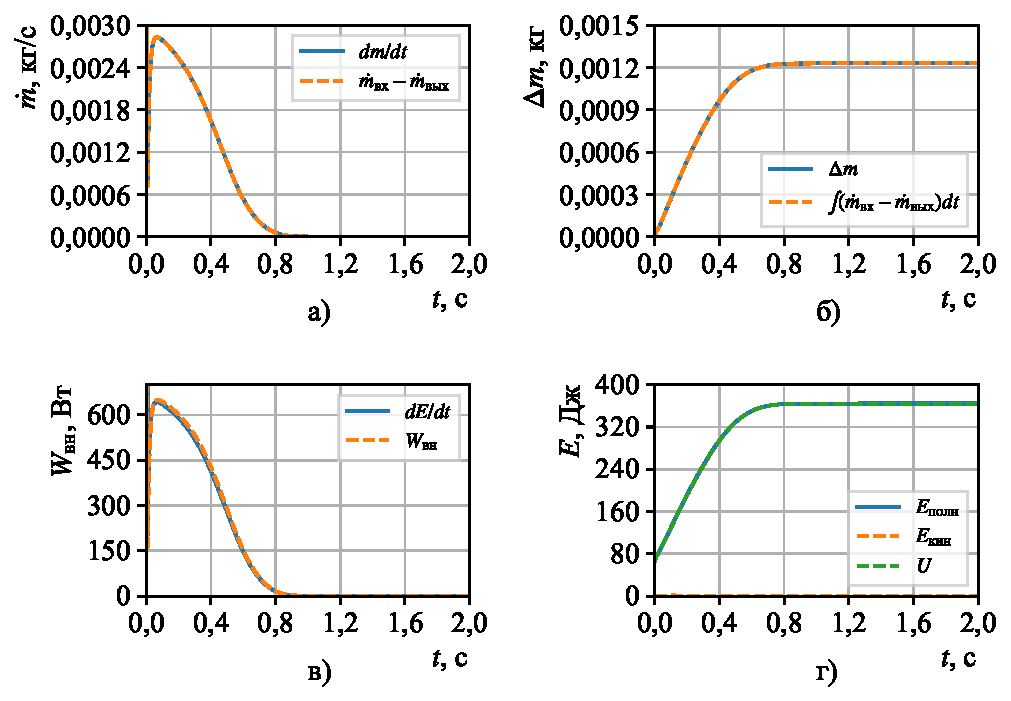
\includegraphics{part2/conservation_laws_verification.pdf}
    }
    \caption{Энергетический баланс системы при различных состояниях распределителей}
    \label{fig:ch2/energy_balance}

\end{figure}

В таблице \ref{tab:ch2/energy_balance} представлены относительная ошибка
энергетического баланса и закона сохранения массы
для всех рассмотренных режимов работы системы.

\begin{table}[h]
    \centering
    \caption{Относительная погрешность энергетического баланса и закона сохранения массы}
    \begin{tabular}{l|c|c}
        \midrule
        № описания & Погрешность энергии, \% & Погрешность массы, \% \\
        \midrule
        1          & \num{0.0084}                  & \num{0.3203}                \\
        \hline
        2          & \num{0.0217}                  & \num{0.9068}                \\
        \hline
        3          & \num{0.0029}                  & \num{0.4324}                \\
        \hline
        4          & \num{0.0002}                  & \num{0.2321}                \\
        \hline
        5          & \num{0.0052}                  & \num{0.8042}                \\
        \hline
        6          & \num{0.0018}                  & \num{0.3963}                \\
        \midrule
    \end{tabular}
    \label{tab:ch2/energy_balance}
\end{table}

\paragraph{Оценка физической непротиворечивости уравнений.} 
Рассмотрение соблюдение второго начала термодинамики так же проводилось для всех режимов работы системы. На рисунке
\ref{fig:ch2/thermodynamics_analysis} представлены результаты термодинамического анализа процессов в пневмоприводе 
для режима 2. Остальные режимы представлены в приложении к \fixme{диссертации}.

\begin{figure}[ht]
    \centerfloat {
        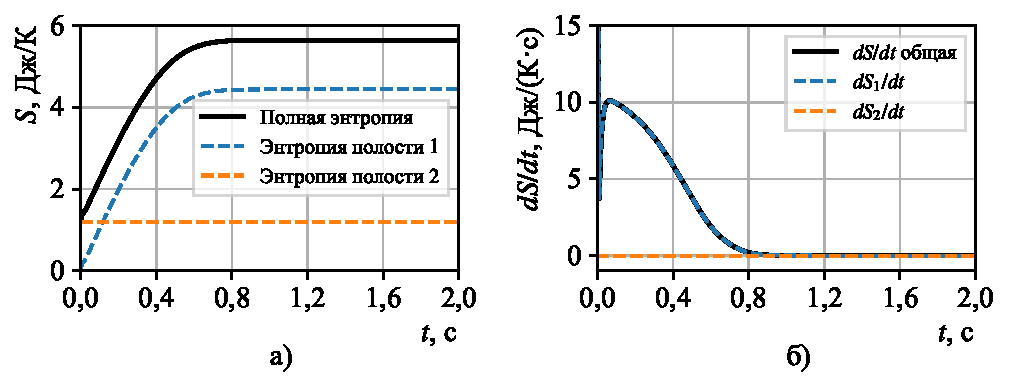
\includegraphics{part2/thermodynamic_analysis.pdf}
    }
    \caption{Комплексный термодинамический анализ процессов в полостях электропневматического привода с дискретными распределителями}
    \label{fig:ch2/thermodynamics_analysis}

\end{figure}

Анализ динамики изменения энтропии
демонстрирует положительную скорость изменения суммарной 
энтропии системы $dS_{сумм}/dt$, что подтверждает соблюдение второго начала термодинамики.
Максимальная скорость роста энтропии наблюдается в начальный момент времени и составляет порядка 
20 \si{\joule\per\kelvin\per\second}, что обусловлено интенсивными процессами массообмена при открытии распределителя
в левой полости пневмоцилиндра.

График эволюции полной энтропии отражает монотонный рост суммарной энтропии системы~$S_{сумм}$~с последующим 
выходом на установившееся значение около 5~\si{\joule\per\kelvin}. 

Представленные результаты термодинамического анализа подтверждают корректность
разработанной математической модели электропневматического привода с точки зрения соблюдения 
фундаментальных законов термодинамики и позволяют детально исследовать характер протекающих в системе процессов.

\subsection{Заключение о достоверности модели}\label{sec:ch2/sec6/subsec5}

Проведенная верификация математической модели электропневматического привода подтвердила её адекватность и достоверность.
Анализ размерностей и единиц измерения продемонстрировал корректность математических формулировок всех уравнений модели.
Проверка согласованности с фундаментальными законами физики показала, что относительная погрешность соблюдения
закона сохранения энергии не превышает \num{0.007} процентов, а закона сохранения массы~---~\num{0.91} процентов
для всех исследованных режимов работы.
Термодинамический анализ подтвердил соблюдение второго начала термодинамики,
что проявляется в положительной скорости изменения суммарной энтропии системы с максимальным значением
около \SI{20}{\joule\per\kelvin\per\second} в начальный момент времени. Анализ температурно-энтропийных
и p-v диаграмм показал физически корректное описание термодинамических процессов в полостях пневмоцилиндра.

Таким образом, комплексная верификация подтверждает, что разработанная математическая модель
корректно описывает все существенные физические процессы в электропневматическом приводе с
дискретными распределителями и может быть использована для решения задач анализа и синтеза систем управления.